\ProvidesFile{tests.tex}

\section{Тестирование}
Проведено тестирование на корректность и на устойчивость для всех реализованных в данном руководстве классов, поэтому все имплементированные классы являются корректными. Тесты, как и способы их запустить, находятся в этом же репозитории.

\subsection{Длинка}
Отдельно хочется сравнить скорость выполнения операций у самописного класса uint\_t относительно скорости длинки от буста. Характеристики машины:
\begin{itemize}
  \item Процессор: 12th Gen Intel(R) Core(TM) i7-12700K
  \item Видеокарта: GeForce RTX 3060 Ti Lite Hash Rate
  \item Оперативная память: DDR4, 8 ГБx2, 2400 МГц,
\end{itemize}
Вот результаты замеров времени работы при одинаковой нагрузке:
\begin{itemize}
  \item Debug сборка:

  \begin{center}
     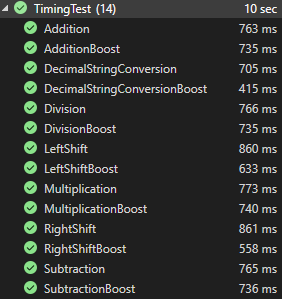
\includegraphics{images/uint_debug.png}
  \end{center}

  \item Release сборка:

  \begin{center}
     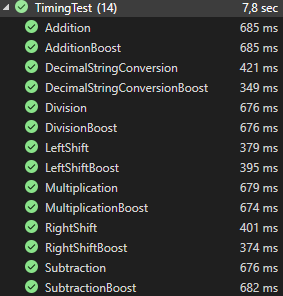
\includegraphics{images/uint_release.png}
  \end{center}
\end{itemize}

Мы сравнялись почти во всех операциях. Это достаточно неплохой результат, поэтому можно продолжать использование данного класса, не забывая о возможности дальнейших оптимизаций данного класса.

\subsection{Эль-Гамаль}
Результаты времени работы Эль-Гамаля для 1000 сообщений из 128 бит над NIST P-256:
\begin{itemize}
  \item Debug сборка:

    TODO

  \item Release сборка:

    TODO
\end{itemize}
Так как никто из нормальных людей не использует Эллиптического Эль-Гамаля, то придётся сравнить его с \href{https://github.com/RustCrypto/elliptic-curves/tree/master/p256}{Эллиптическим Диффи-Хеллманом}, который написан на расте:

\begin{center}
  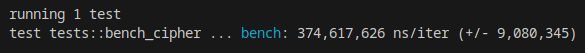
\includegraphics{images/outsource_elgamal.png}
\end{center}

То есть он выполнился за $\thicksim 375$ мс ($\pm9$ мс). При одинаковых условиях TODO

\subsection{ECDSA}
Результаты времени работы Эль-Гамаля для 1000 сообщений из 128 бит над NIST P-256:
\begin{itemize}
  \item Debug сборка:

    TODO

  \item Release сборка:

    TODO
\end{itemize}

Раз уж мы использовали \href{https://github.com/RustCrypto/elliptic-curves/tree/master/p256}{эту библиотеку}, то можно сравнить именно с её ECDSA:

\begin{center}
  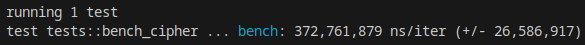
\includegraphics{images/outsoucre_ecdsa.png}
\end{center}

Как видим, результаты $\thicksim 372$ мс ($\pm26$ мс). При одинаковых условиях TODO

